\documentclass{tufte-handout}
%------------------------------------------------
%\geometry{showframe} % display margins for debugging page layout
%------------------------------------------------
\usepackage{graphicx} % allow embedded images
  \setkeys{Gin}{width=\linewidth,totalheight=\textheight,keepaspectratio}
  \graphicspath{{/home/swl/Dropbox/ucd/eu_economics/figs/}}  % set of paths to search for images
\usepackage{amsmath}  % extended mathematics
\usepackage{booktabs} % book-quality tables
\usepackage{units}    % non-stacked fractions and better unit spacing
\usepackage{multicol} % multiple column layout facilities
\usepackage{lipsum}   % filler text
\usepackage{fancyvrb} % extended verbatim environments
  \fvset{fontsize=\normalsize}% default font size for fancy-verbatim environments

%------------------------------------------------
% Standardize command font styles and environments
\newcommand{\doccmd}[1]{\texttt{\textbackslash#1}}% command name -- adds backslash automatically
\newcommand{\docopt}[1]{\ensuremath{\langle}\textrm{\textit{#1}}\ensuremath{\rangle}}% optional command argument
\newcommand{\docarg}[1]{\textrm{\textit{#1}}}% (required) command argument
\newcommand{\docenv}[1]{\textsf{#1}}% environment name
\newcommand{\docpkg}[1]{\texttt{#1}}% package name
\newcommand{\doccls}[1]{\texttt{#1}}% document class name
\newcommand{\docclsopt}[1]{\texttt{#1}}% document class option name
\newenvironment{docspec}{\begin{quote}\noindent}{\end{quote}}% command specification environment
%------------------------------------------------

%------------------------------------------------
%%%% Details %%%%
%------------------------------------------------
\title{EU Economics: Brexit}
\author{University College Dublin}
\date{Spring 2017} 

\begin{document}
\maketitle  
% BREXIT

%------------------------------------------------
% FIGURE: 
\begin{figure} \centering
    \includegraphics[scale=.3]{pound_exchange.png}
    \caption{Pound exchange rate relative to the Euro for 2016. Note that the graph covers time-series data for trading days only. Data: Eurostat}
    \label{fig:pound}
  \end{figure}
%------------------------------------------------

%------------------------------------------------
% FIGURE: 
\begin{figure} \centering
    \includegraphics[scale=.3]{uk_eu_trade.png}
    \caption{UK trade, imports from and exports to, other EU member statesData: HM Revenue and Customs}
    \label{fig:uk_trade1}
  \end{figure}
%------------------------------------------------

%------------------------------------------------
% FIGURE: 
\begin{figure} \centering
    \includegraphics[scale=.3]{uk_tradeq.png}
    \caption{Trade per quarter with other EU member states and the rest of the world. Data: HM Revenue and Customs}
    \label{fig:uk_trade2}
  \end{figure}
%------------------------------------------------


%------------------------------------------------
% FIGURE: 
\begin{figure} \centering
    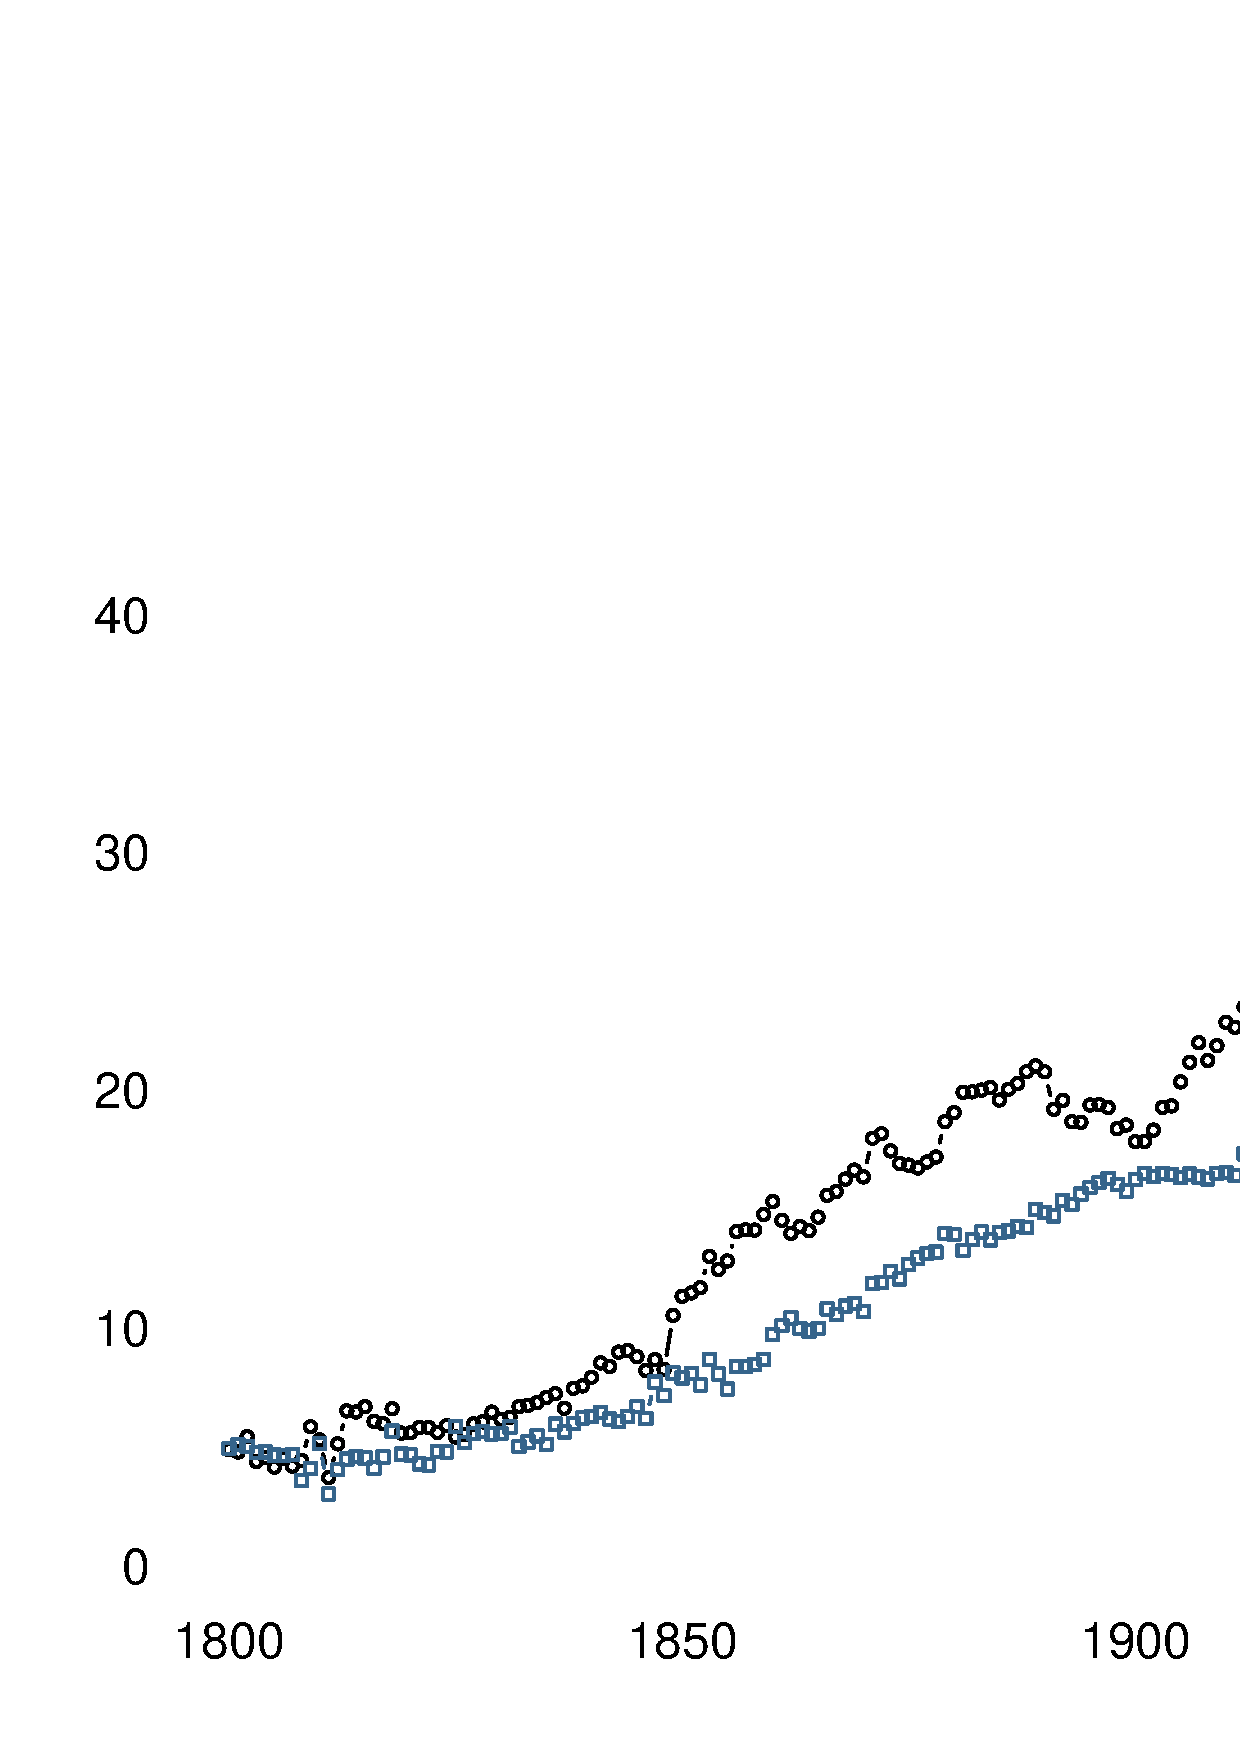
\includegraphics[scale=.3]{uk_trade.png}
    \caption{UK imports and exports with global partners. EU states are represented by the black squares. Data: HM Revenue and Customs}
    \label{fig:uk_trade3}
  \end{figure}
%------------------------------------------------
%------------------------------------------------------------------------------
\end{document}
